\documentclass{ctexart} 
\usepackage[utf8]{inputenc}
\usepackage{amsmath}
\usepackage{graphicx}
\usepackage{listings}
\usepackage{array}
\usepackage{indentfirst}
\usepackage{xcolor}
\usepackage{geometry}
\usepackage{setspace}
\usepackage{float}
\usepackage{algpseudocode}
\usepackage{caption}
\usepackage{hyperref}
\usepackage{algorithm}

\usepackage{tikz}
\usetikzlibrary{er, positioning, arrows.meta}


\lstset{
    language=Java,
    basicstyle=\ttfamily\small,
    breaklines=true,
    frame=single,
    numbers=left,
    numberstyle=\tiny\color{gray},
    keywordstyle=\color{blue},
    commentstyle=\color{green},
    stringstyle=\color{red},
    showstringspaces=false
}

\begin{document}
\title{\fontsize{35pt}{\baselineskip}\selectfont\linespread{2}\selectfont{\textbf{基于MySQL的精简图书管理系统}}}

\date{\huge{\today}}
\author{\large\textbf{叶容宇 3230101885}}
\maketitle

\begin{figure}[ht]
    \centering
    
\includegraphics[scale=0.5]{ZJU.jpg}
\end{figure}

\maketitle
\newpage
\tableofcontents
\newpage
\section{实验目的}
本实验旨在设计并实现一个图书管理系统的数据库,该系统能够有效地管理图书、借阅者卡片以及借阅记录,并通过一系列的测试用例来验证系统的正确性和性能。
最终目的是提供一个基于MySQL的精简图书管理程序,该图书管理程序应具备较好的可扩展性、鲁棒性和安全性,并且在高并发场景下仍能正确运行。

\section{实验环境}

本实验基于MySQL数据库,使用Java语言进行编程。

前端使用Vue.js,后端使用Spring Boot框架。

在Windows环境下

启动后端

\texttt{mvn spring-boot:run}

启动前端(在librarymanagementsystem-frontend目录下)

\texttt{npm run dev}

运行所有的测试

\texttt{mvn -Dtest=LibraryTest clean test}
\section{项目文件结构}

本项目采用Maven项目结构,主要包含以下几个模块:

\begin{itemize}
    \item \texttt{src/main/java}: 包含Java源代码。
    \item \texttt{src/main/resources}: 包含配置文件,如数据库连接信息。
    \item \texttt{src/test/java}: 包含测试代码。
    \item \texttt{librarymanagementsystem-frontend}: 前端代码。
    \item \texttt{report}: 实验报告及相关文档。
\end{itemize}

在 \texttt{src/main/java} 目录下,主要模块如下:

\begin{itemize}
    \item \texttt{config}: 配置文件,如跨域配置。
    \item \texttt{entities}: 实体类,如书籍、借阅者卡片等。
    \item \texttt{queries}: 查询条件和结果类。
    \item \texttt{library.system}: 核心系统类和接口。
    \item \texttt{library.system.controller}: 控制器层,负责处理前端请求。
    \item \texttt{utils}: 工具类。
\end{itemize}

\section{文件作用说明}

\subsection{\texttt{config/CorsConfig.java}}
文件定义了跨域资源共享(CORS)的配置,以允许前端应用从不同的源访问API,确保前后端协同工作时不会遇到跨域问题。
在实验中最初发现前后端不能完成正常通信。前端发送的请求会被后端404拒绝,原因是没有配置spring boot的跨域规则。

\textbf{功能说明:}
\begin{itemize}
    \item 使用\texttt{@Configuration}注解标记为配置类。
    \item 通过\texttt{@Bean}注解定义了一个\texttt{CorsFilter} Bean,用于处理跨域请求。
    \item 配置允许所有来源(\texttt{"*"})、所有请求头(\texttt{"*"})和所有HTTP方法(\texttt{"*"}),并允许凭据(\texttt{setAllowCredentials(true)})。
\end{itemize}

\textbf{代码关键点:}
\begin{itemize}
    \item \texttt{CorsConfiguration}用于定义跨域规则。
    \item \texttt{UrlBasedCorsConfigurationSource}用于将跨域规则绑定到特定的URL路径(\texttt{"**"}表示所有路径)。
    \item \texttt{CorsFilter}用于实际拦截请求并应用跨域规则。
\end{itemize}

\textbf{设计思路:}
\begin{itemize}
    \item 确保前后端分离时,前端可以无限制地访问后端API。
    \item 在开发和测试阶段,允许所有来源的访问以简化调试。
\end{itemize}

\begin{lstlisting}[caption=\texttt{config/CorsConfig.java}]
package config;

import org.springframework.context.annotation.Bean;
import org.springframework.context.annotation.Configuration;
import org.springframework.web.cors.CorsConfiguration;
import org.springframework.web.cors.UrlBasedCorsConfigurationSource;
import org.springframework.web.filter.CorsFilter;

@Configuration
public class CorsConfig {
    private static final long MAX_AGE = 24 * 60 * 60; // 1 day

    @Bean
    public CorsFilter corsFilter() {
        UrlBasedCorsConfigurationSource source = new UrlBasedCorsConfigurationSource();
        CorsConfiguration config = new CorsConfiguration();
        config.addAllowedHeader("*");
        config.addAllowedMethod("*");
        config.addAllowedOrigin("http://localhost:5173");
        config.setMaxAge(MAX_AGE);
        source.registerCorsConfiguration("/**", config);
        return new CorsFilter(source);
    }
}

\end{lstlisting}

\subsection{\texttt{src/main/java/library/system/LibraryManagementSystem.java}}
文件定义了图书管理系统的接口,声明了系统需要实现的各种功能,如注册图书、借书、还书等。
通过\texttt{PreparedStatement}预编译SQL语句,避免SQL注入攻击。
使用\texttt{stmt.executeUpdate()}执行SQL语句,与数据库交互。
\textbf{功能说明:}
\begin{itemize}
    \item 定义了系统的核心功能接口,包括:
      \begin{itemize}
          \item \texttt{storeBook(Book book)}:注册新图书。
          \item \texttt{borrowBook(Borrow borrow)}:借书。
          \item \texttt{returnBook(Borrow borrow)}:还书。
          \item \texttt{storeBook(List<Book> books)}:批量注册图书。
          \item \texttt{queryBook(BookQueryConditions conditions)}:查询图书。
      \end{itemize}
\end{itemize}

\textbf{代码关键点:}
\begin{itemize}
    \item 使用\texttt{ApiResult}作为返回值,统一处理成功和失败的响应。
    \item \texttt{BookQueryResults}用于封装查询结果,包含状态、消息和图书列表。
\end{itemize}

\textbf{设计思路:}
\begin{itemize}
    \item 通过接口定义系统功能,便于后续实现和扩展。
    \item 使用统一的返回类型(\texttt{ApiResult}和\texttt{BookQueryResults})简化前端处理逻辑。
\end{itemize}

\begin{lstlisting}[caption=\texttt{library.system/LibraryManagementSystem.java}]
public interface LibraryManagementSystem {

    ApiResult storeBook(Book book);
    ApiResult incBookStock(int bookId, int deltaStock);
    ApiResult storeBook(List<Book> books);
    ApiResult removeBook(int booApiResultkId);
    ApiResult queryBook(BookQueryConditions conditions);
    ApiResult borrowBook(Borrow borrow);
    ApiResult returnBook(Borrow borrow);
    ApiResult showBorrowHistory(int cardId);
    ApiResult registerCard(Card card);
    ApiResult removeCard(int cardId);
    ApiResult showCards();
    ApiResult modifyCardInfo(Card card);
}
\end{lstlisting}

\subsection{\texttt{src/main/java/library/system/LibraryManagementSystemImpl.java}}
文件实现了\texttt{LibraryManagementSystem}接口,提供了具体的功能实现。
在进行并行请求测试的时候使用\texttt{FOR UPDATE}锁定记录,避免数据不一致的问题。

\textbf{功能说明:}
\begin{itemize}
    \item 实现了\texttt{LibraryManagementSystem}接口的所有方法。
    \item 完成了图书注册、图书批量注册、并发借阅、借阅和还书等功能。
\end{itemize}

\textbf{设计思路:}
\begin{itemize}
    \item 使用\texttt{PreparedStatement}预编译SQL语句,避免SQL注入攻击。
    \item 使用统一的返回类型
\end{itemize}

\begin{lstlisting}[caption=\texttt{library.system/LibraryManagementSystemImpl.java}]
import org.springframework.stereotype.Component;
import org.springframework.stereotype.Service;

@Component
@Service
public class LibraryManagementSystemImpl implements LibraryManagementSystem {

    private final DatabaseConnector connector;

    public LibraryManagementSystemImpl(DatabaseConnector connector) {
        this.connector = connector;
    }

    @Override
    public ApiResult storeBook(Book book) {
        Connection conn = connector.getConn();
        try {
            PreparedStatement checkStmt = conn.prepareStatement(
                    "SELECT COUNT(*) FROM book WHERE category = ? AND title = ? AND press = ? AND author = ? AND publish_year = ?");
            checkStmt.setString(1, book.getCategory());
            checkStmt.setString(2, book.getTitle());
            checkStmt.setString(3, book.getPress());
            checkStmt.setString(4, book.getAuthor());
            checkStmt.setInt(5, book.getPublishYear());

            ResultSet rs = checkStmt.executeQuery();
            rs.next();
            int count = rs.getInt(1);

            if (count > 0) {
                return new ApiResult(false, "Book already exists in the library system.");
            }

            PreparedStatement insertStmt = conn
                    .prepareStatement(
                            "INSERT INTO book (category, title, press, publish_year, author, price, stock) VALUES (?,?,?,?,?,?,?)",
                            Statement.RETURN_GENERATED_KEYS);
            insertStmt.setString(1, book.getCategory());
            insertStmt.setString(2, book.getTitle());
            insertStmt.setString(3, book.getPress());
            insertStmt.setInt(4, book.getPublishYear());
            insertStmt.setString(5, book.getAuthor());
            insertStmt.setDouble(6, book.getPrice());
            insertStmt.setInt(7, book.getStock());

            int affectedRows = insertStmt.executeUpdate();
            if (affectedRows == 1) {
                ResultSet generatedKeys = insertStmt.getGeneratedKeys();
                if (generatedKeys.next()) {
                    book.setBookId(generatedKeys.getInt(1));
                }
                commit(conn);
                return new ApiResult(true, "Book stored successfully");
            } else {
                rollback(conn);
                return new ApiResult(false, "Failed to store book");
            }

        } catch (Exception e) {
            rollback(conn);
            return new ApiResult(false, e.getMessage());
        }
    }

\end{lstlisting}

\subsection{\texttt{src/main/java/library/system/controller/BookController.java}}
文件是控制器层的一部分,处理与图书相关的HTTP请求,如注册新图书、查询图书等。

\textbf{功能说明:}
\begin{itemize}

    \item 使用\texttt{@RestController}注解标记为控制器。
    \item 使用\texttt{@RequestMapping("/api")}定义了API的基路径。
\end{itemize}

\textbf{设计思路:}
\begin{itemize}
    \item 通过\texttt{@RequestBody}和\texttt{@RequestParam}注解解析请求参数。
    \item 将业务逻辑委托给\texttt{LibraryManagementSystem}接口实现类,保持控制器的简洁性。
\end{itemize}

\begin{lstlisting}[caption=\texttt{library.system.controller/BookController.java}]
import org.springframework.beans.factory.annotation.Autowired;
import org.springframework.web.bind.annotation.*;

@RestController
@CrossOrigin(origins = "http://localhost:5173")
@RequestMapping("/api")
public class BookController {
    @Resource
    private LibraryManagementSystem library;
    private static final Logger log = Logger.getLogger(BookController.class.getName());

    @PostConstruct
    public void init() {
        try {
            ConnectConfig conf = new ConnectConfig();
            DatabaseConnector connector = new DatabaseConnector(conf);
            boolean connStatus = connector.connect();
            if (!connStatus) {
                throw new SQLException("Failed to connect to database.");
            }
            this.library = new LibraryManagementSystemImpl(connector);
        } catch (Exception e) {
            throw new RuntimeException("Failed to initialize the controller.", e);
        }
        resetDatabase();

    }

    public BookController() {
        init();
    }

    @GetMapping("/book")
    public BookQueryResults queryBooks(@ModelAttribute BookQueryConditions queryConditions) {
        try {
            ApiResult result = library.queryBook(queryConditions);
            if (!result.ok) {
                throw new RuntimeException("Failed" + result.message);
            }
            return (BookQueryResults) result.payload;
        } catch (Exception e) {
            throw new RuntimeException("Failed to query books.", e);
        }
    }
}
\end{lstlisting}

\section{实验结果}
\subsection{测试用例验证}
最终的测试用例验证了系统的正确性和性能,成功通过了\texttt{LibraryTest}中的所有测试函数
\begin{lstlisting}
    [INFO] Tests run: 9, Failures: 0, Errors: 0, Skipped: 0, Time elapsed: 18.576 s - in LibraryTest
    [INFO] 
    [INFO] Results:
    [INFO]
    [INFO] Tests run: 9, Failures: 0, Errors: 0, Skipped: 0
    [INFO]
\end{lstlisting}

\subsection{前后端交互}
\subsubsection{图书查询 出借 注册}
\begin{figure}[h]
    \centering
    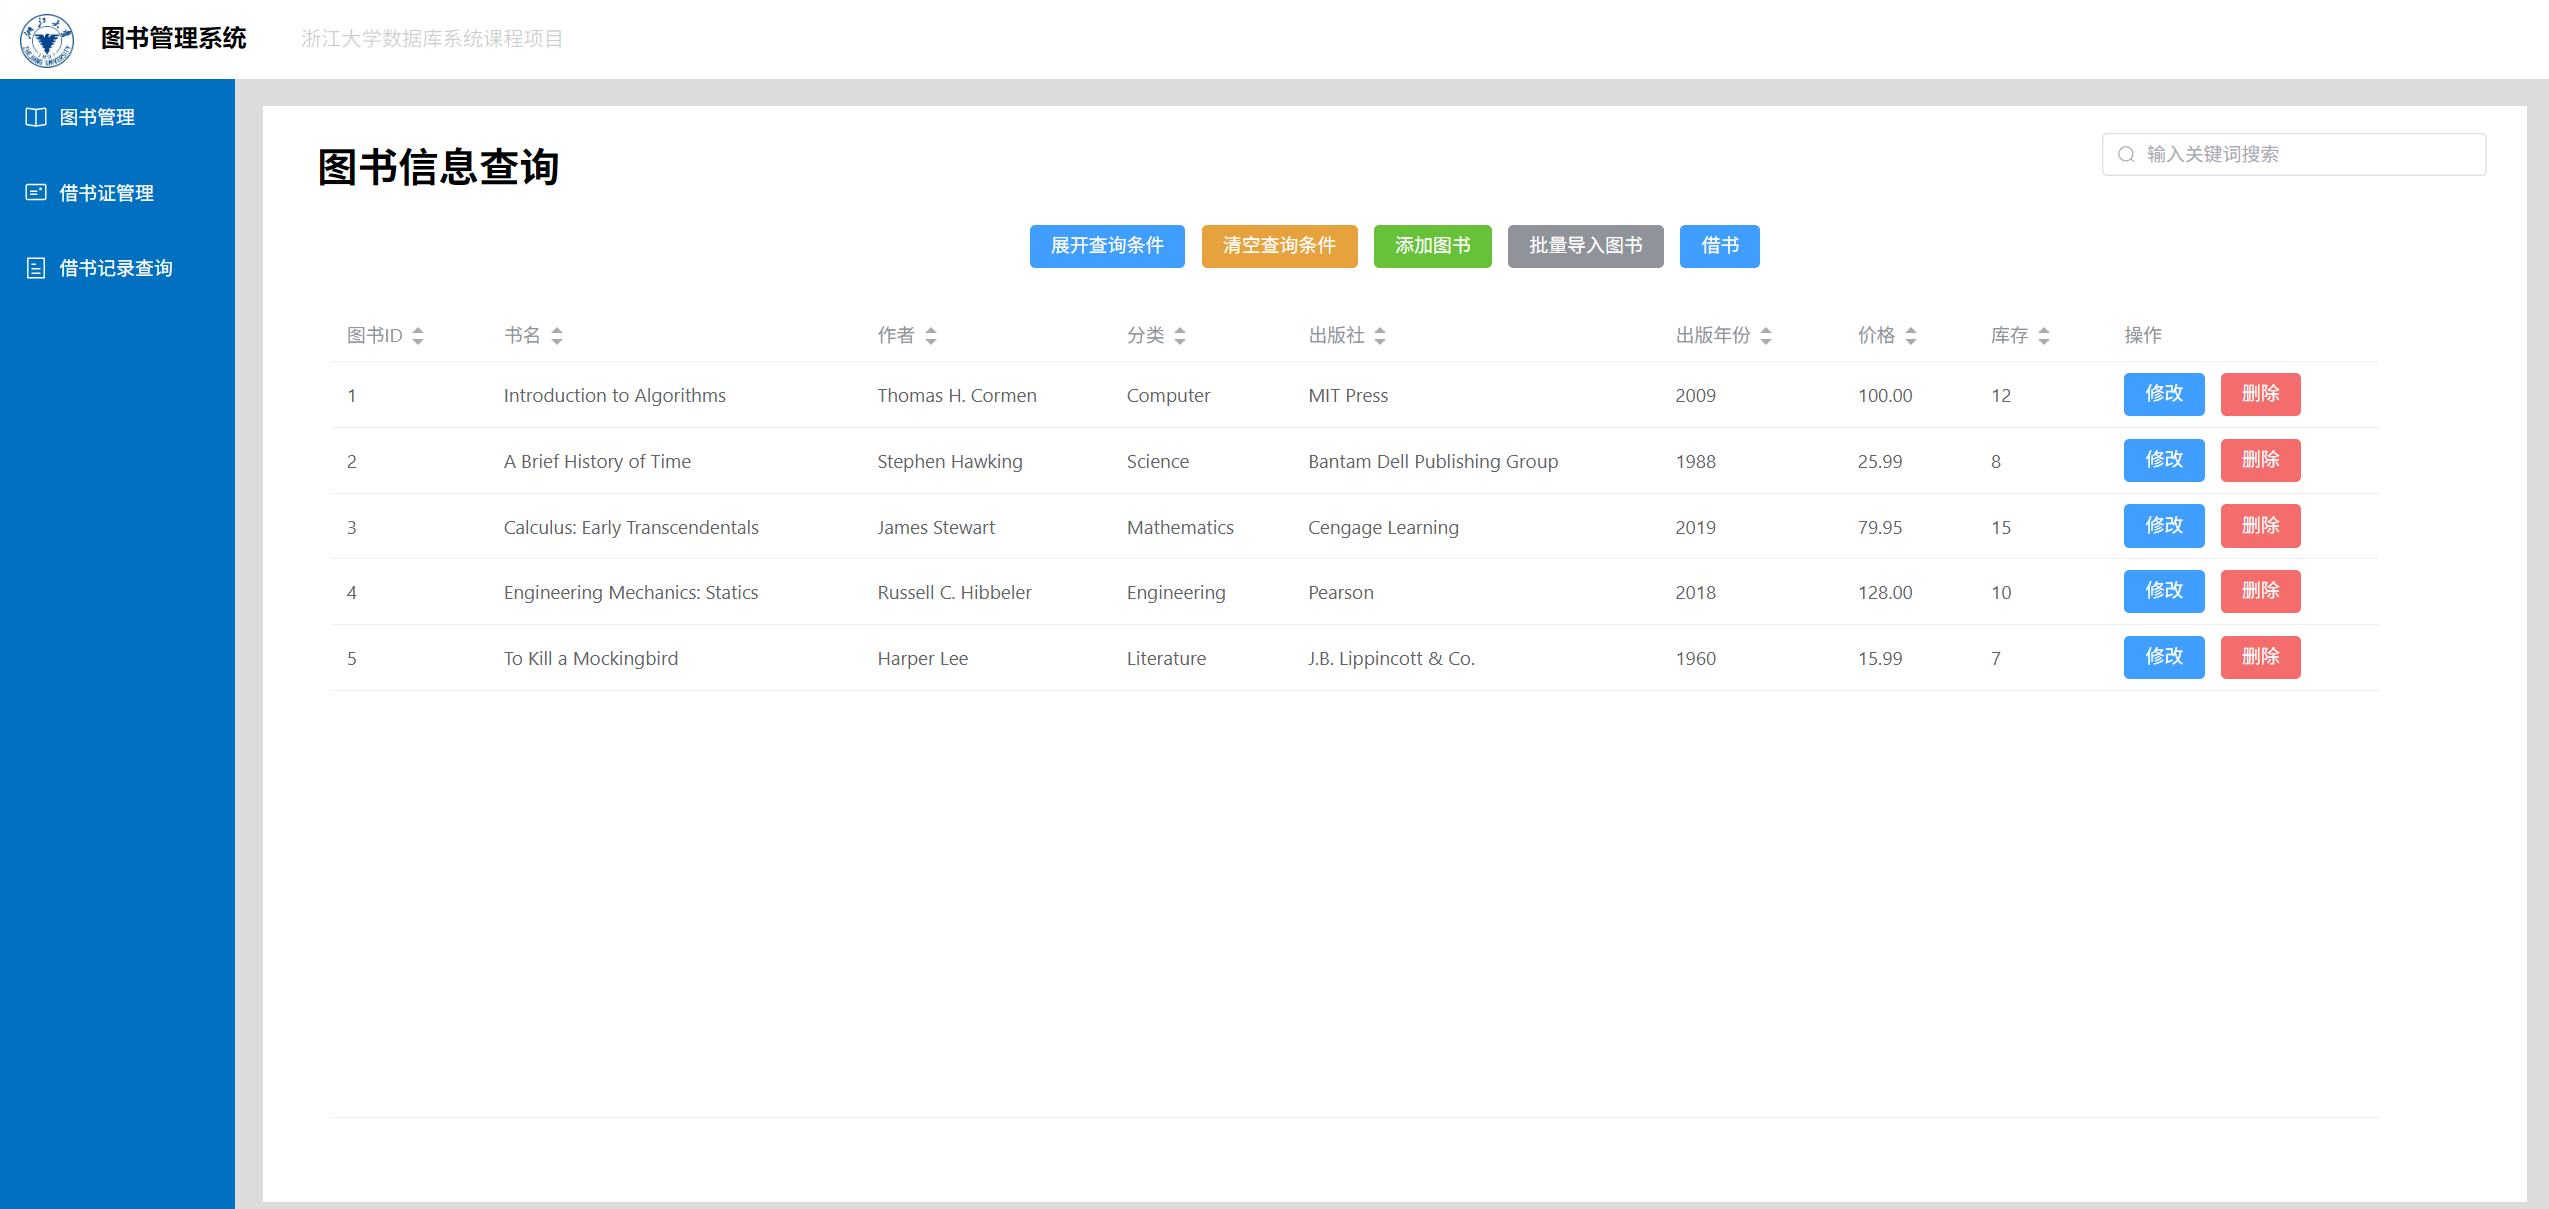
\includegraphics[width=0.8\textwidth]{pic1.png}
    \caption{图书查询界面}
    \label{fig:book-query-borrow-register}
\end{figure}
提供按条件查询按钮。提供导入单本或者批量导入的支持
\subsubsection{借书卡管理}
\begin{figure}[h]
    \centering
    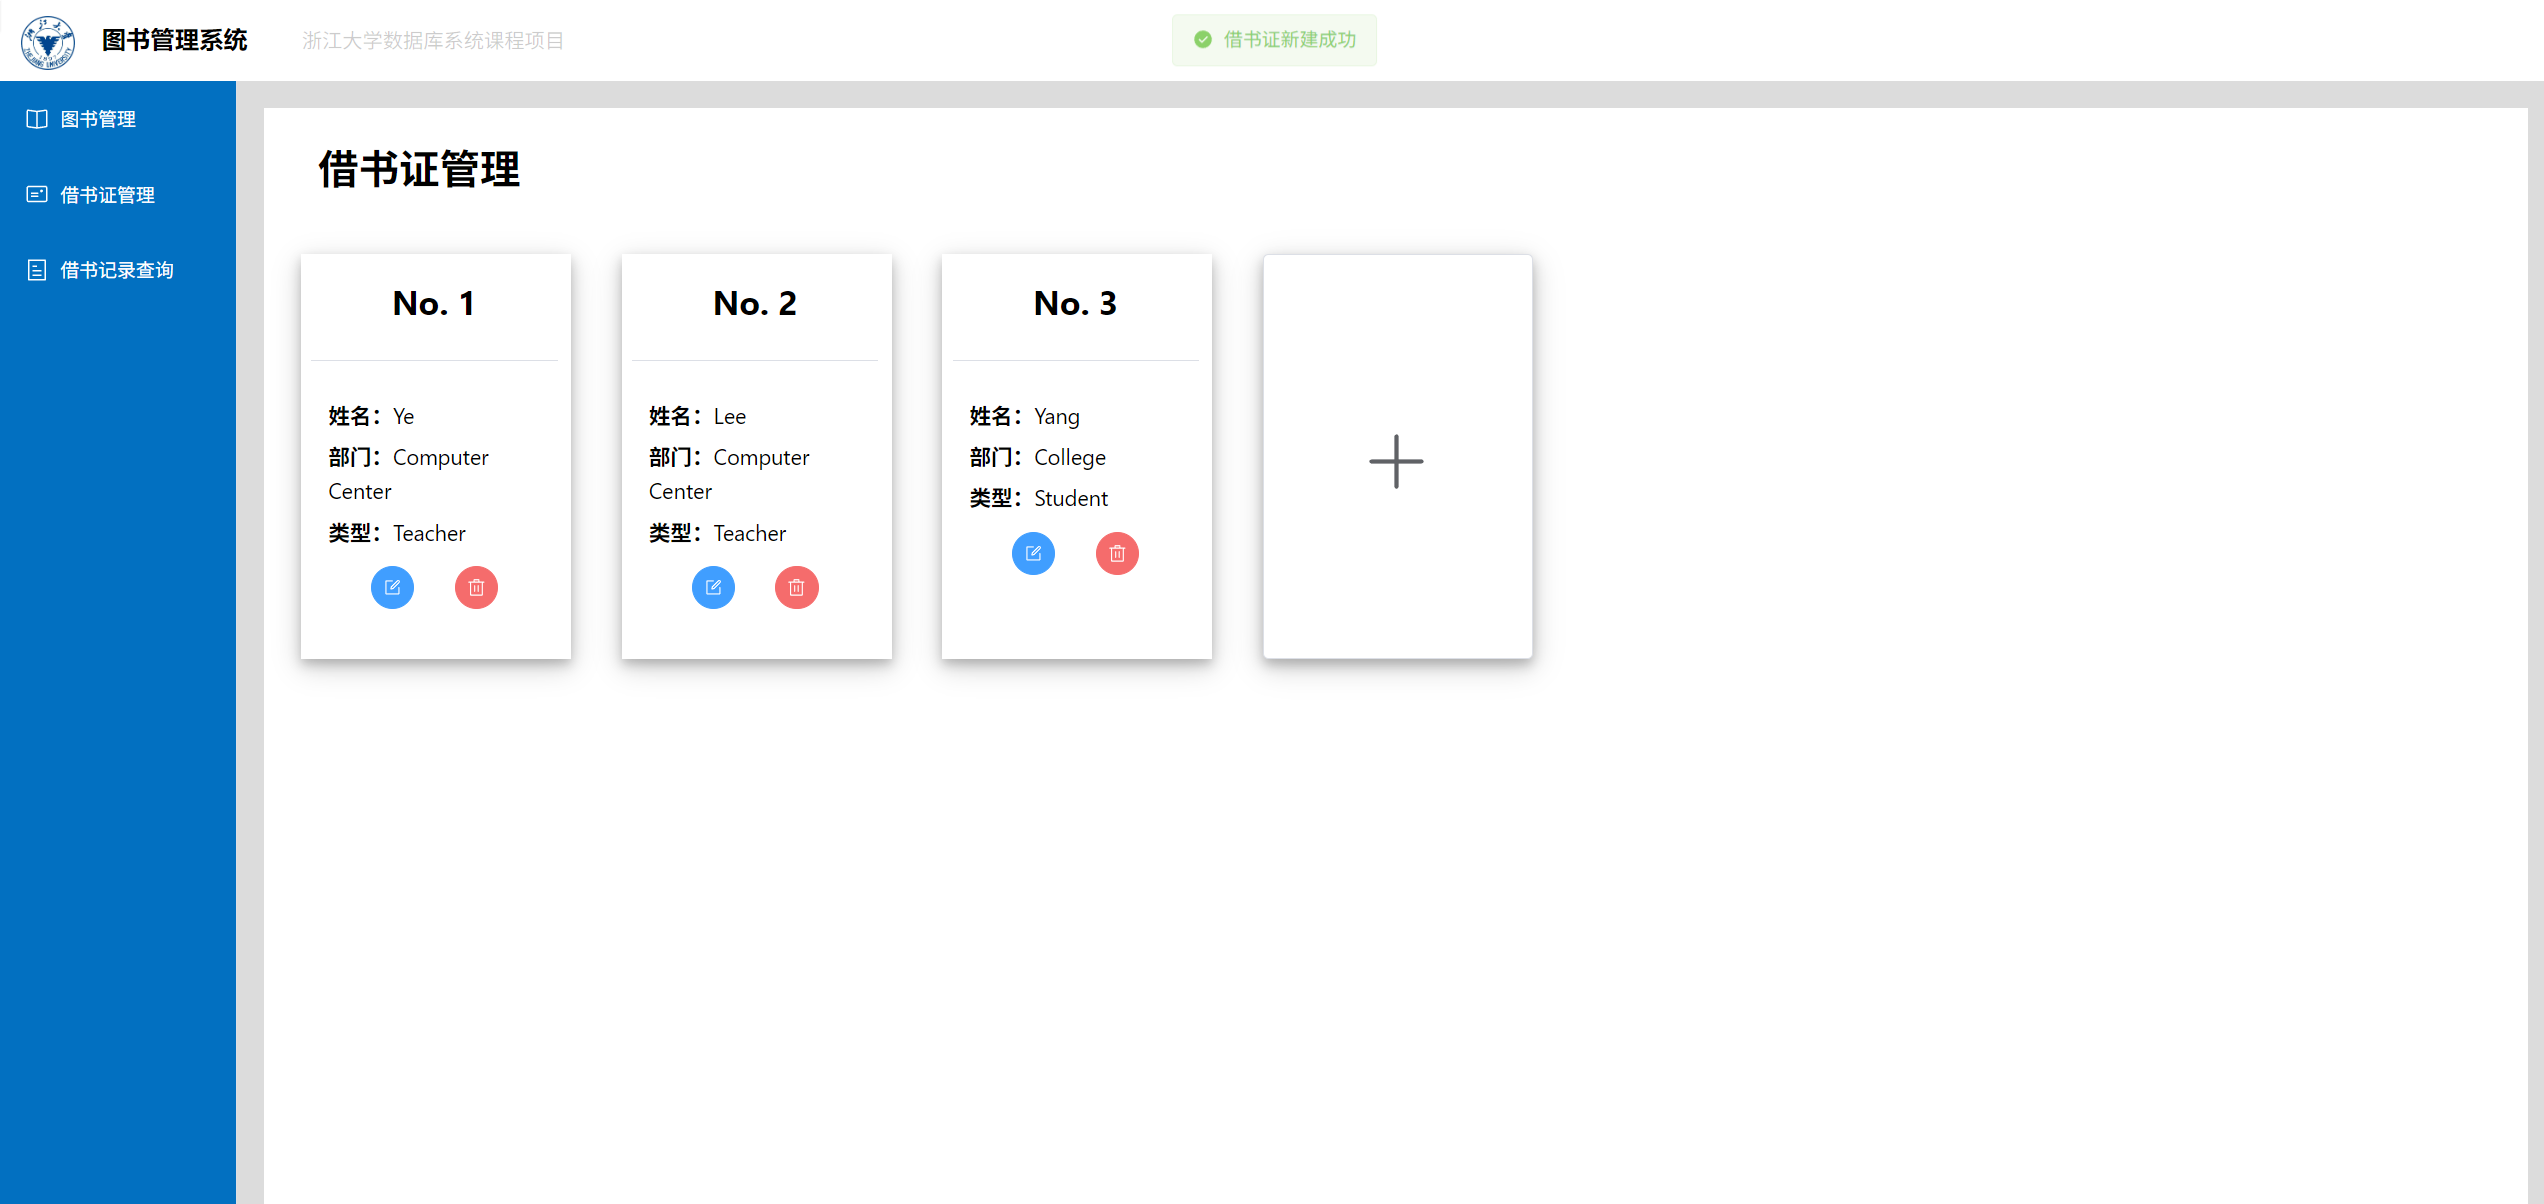
\includegraphics[width=0.8\textwidth]{pic2.png}
    \caption{借书卡管理界面}
    \label{fig:library-card-management}
\end{figure}
查询所有的借书卡,编辑、删除、新增借书卡。
\newpage
\subsubsection{借阅历史}
\begin{figure}[h]
    \centering
    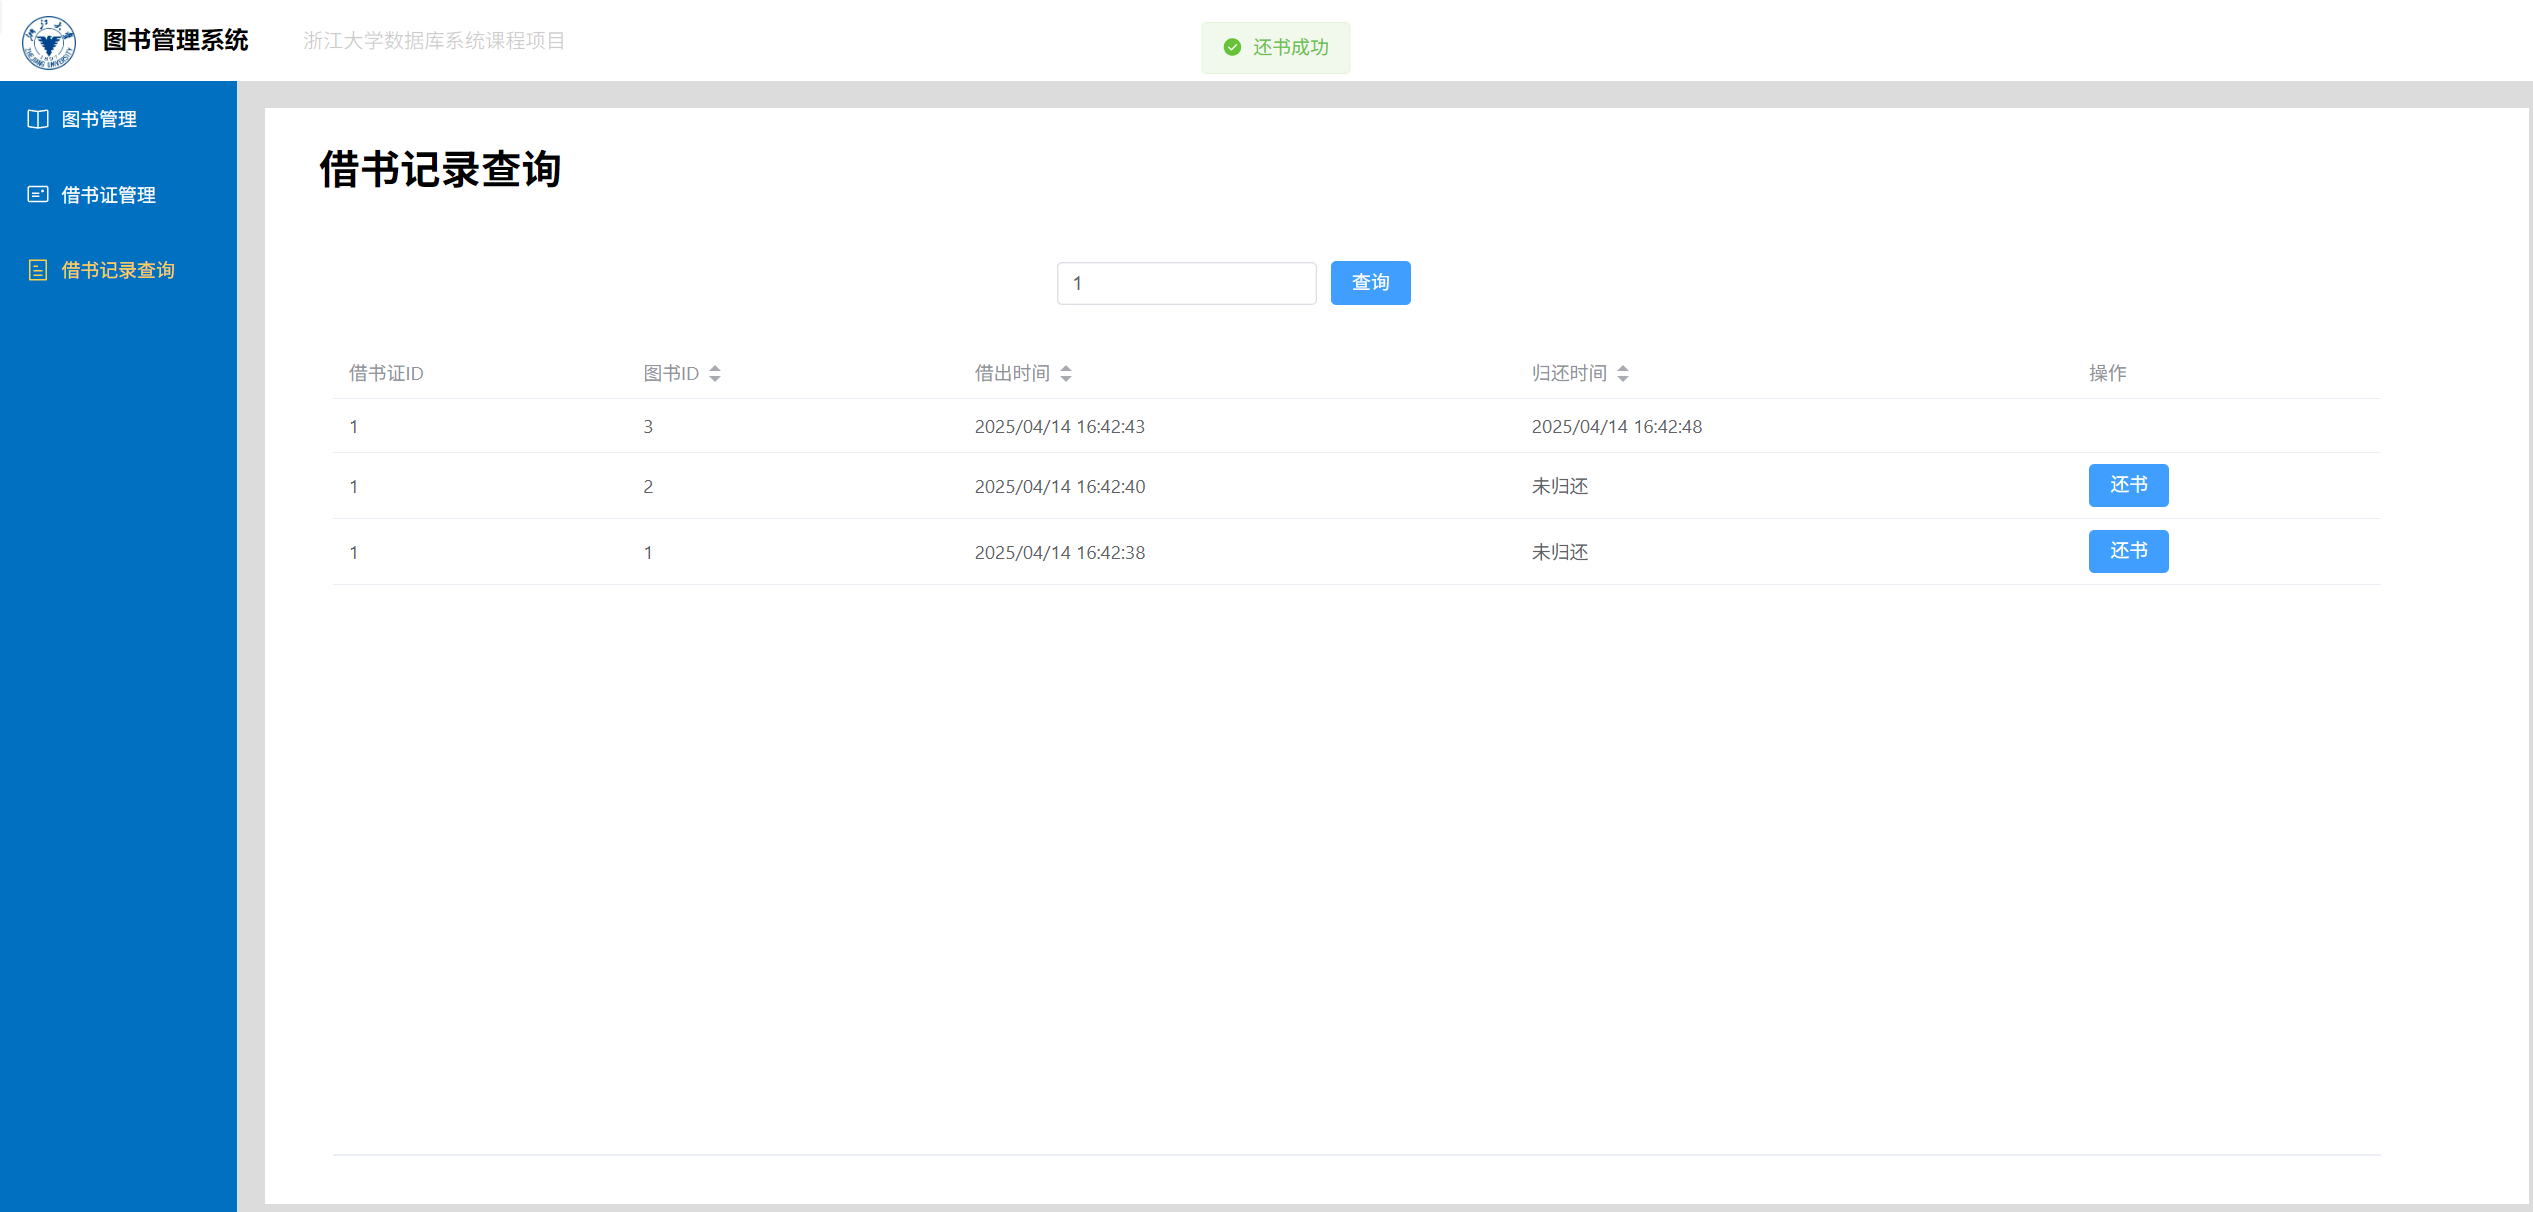
\includegraphics[width=0.8\textwidth]{pic3.png}
    \caption{借阅历史界面}
    \label{fig:borrowing-history}
\end{figure}
可以根据借书卡号查找借阅历史,并且可以手动归还书籍。

\section{思考题}
\begin{tikzpicture}[>=Stealth, node distance=1cm]
    % 定义实体
    \node[entity] (book) {Book (书籍)};
    \node[attribute] (book_id) [below left=of book] {book\_id (主键)} edge (book);
    \node[attribute] (category) [below=of book] {category} edge (book);
    \node[attribute] (title) [below right=of book] {title} edge (book);
    \node[attribute] (press) [right=of book] {press} edge (book);
    \node[attribute] (publish_year) [above right=of book] {publish\_year} edge (book);
    \node[attribute] (author) [above=of book] {author} edge (book);
    \node[attribute] (price) [above left=of book] {price (默认: 0.00)} edge (book);
    \node[attribute] (stock) [left=of book] {stock (默认: 0)} edge (book);

    \node[entity] (card) [below=7cm of book] {Card (借书卡)};
    \node[attribute] (card_id) [below left=of card] {card\_id (主键)} edge (card);
    \node[attribute] (name) [below=of card] {name} edge (card);
    \node[attribute] (department) [below right=of card] {department} edge (card);
    \node[attribute] (type) [right=of card] {type ('T' 或 'S')} edge (card);

    \node[entity] (borrow) [below=3cm of book] {Borrow (借阅记录)};
    \node[attribute] (borrow_card_id) [below left=of borrow] {card\_id (外键)} edge (borrow);
    \node[attribute] (borrow_book_id) [left=of borrow] {book\_id (外键)} edge (borrow);
    \node[attribute] (borrow_time) [below right=of borrow] {borrow\_time (主键)} edge (borrow);
    \node[attribute] (return_time) [right=of borrow] {return\_time (默认: 0)} edge (borrow);

    % 定义关系
    \draw[<->] (book) -- node[above] {1:N} (borrow);
    \draw[<->] (card) -- node[above] {N:1} (borrow);


 
\end{tikzpicture}


\textit{图书管理系统中可能遭受SQL注入攻击的模块:}

借阅模块:用户输入借阅信息时,如果输入验证不严格,可能会被注入恶意SQL代码。
登录和注册模块:用户输入用户名和密码时,如果对输入的特殊字符处理不当,可能会被注入恶意SQL代码。
搜索功能模块:用户输入搜索条件时,如果直接拼接到SQL语句中,可能会被注入恶意SQL代码。

解决方法:使用预编译语句(Prepared Statements)或参数化查询:通过预编译SQL语句,将用户输入的内容作为参数而不是直接拼接在SQL语句中,从而防止SQL注入。

\textit{在InnoDB的默认隔离级别(RR, Repeated Read)下,当出现并发访问时,如何保证借书结果的正确性?}

使用事务:对于借书操作,应将其放在事务中,确保借书、减少库存、记录借阅信息等操作要么全部成功,要么全部失败。
锁机制:在事务中使用锁机制,比如SELECT ... FOR UPDATE,可以锁定正在被查询的记录,防止其他事务对这些记录进行修改,直到当前事务提交或回滚。
\end{document}